\documentclass{theme-2614084}
\usepackage{hyperref}
\usepackage{bookmark}
\usepackage{minted}

\usepackage{hyperref}

% =============================================
% Part 0 信息
% =============================================

\mathsetup{
  % 学生姓名
  student-name = {某同学},
  % 学号
  student-id = {2021xxxx},
  % 院系
  department = {电子与信息工程学院},
  % 专业
  experiment = {实验三 CMOS反相器版图设计},
  % 专业年级
  major = {集成电路设计与集成系统},
  % 日期
  % date = {\today},
}

\begin{document}

% =============================================
% Part 1  封面
% =============================================

\makecover

% =============================================
% Part 2 主文档
% =============================================

\section{实验目的}

\begin{enumerate}
  \item 熟悉 virtuoso editing 设计窗口及操作,熟悉 LSW 窗口
  \item 理解设计库、技术库
  \item 了解 SMIC0.18um 工艺规则
  \item 认识 DRC 设计规则检查,排除错误
\end{enumerate}

\section{实验环境}

\begin{enumerate}
  \item 硬件: PC 机、服务器
  \item 环境:Unix 操作系统、Cadence Virtuoso Editing 版图设计软件
\end{enumerate}

\section{实验内容与步骤}

% (注:按照内容,有截图和说明)

\subsection{实验内容}

\begin{enumerate}
  \item 建立一个技术库。Create a technology library
  \item 建立一个设计库。Create a design library
  \item 建立两个库之间的配属关系。Create attachment between the 2 library
  \item 按照设计规则进行CMOS反相器的版图设计
  \item 进行CMOS反相器的DRC、LVS检查
\end{enumerate}

\subsection{实验步骤}

\subsubsection{准备工作}

输入 \texttt{gvim cds.lib} 并如图所示更新cds.lib的文本内容

\begin{figure}[H]
  \centering
  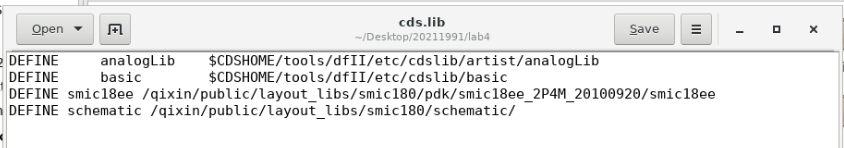
\includegraphics[width=0.6\linewidth]{1-prepare/update-cdslib.png}
  \caption{update cds.lib}
\end{figure}

输入virtuoso\& 并回车,打开virtuoso

在library manager窗口中,确认smic18mmrf在library这一栏里面。勾选Show Categories。新建 Library,并配置 Attach 技术库

\begin{figure}[htbp]
  \centering\begin{minipage}[t]{0.48\textwidth}
      \centering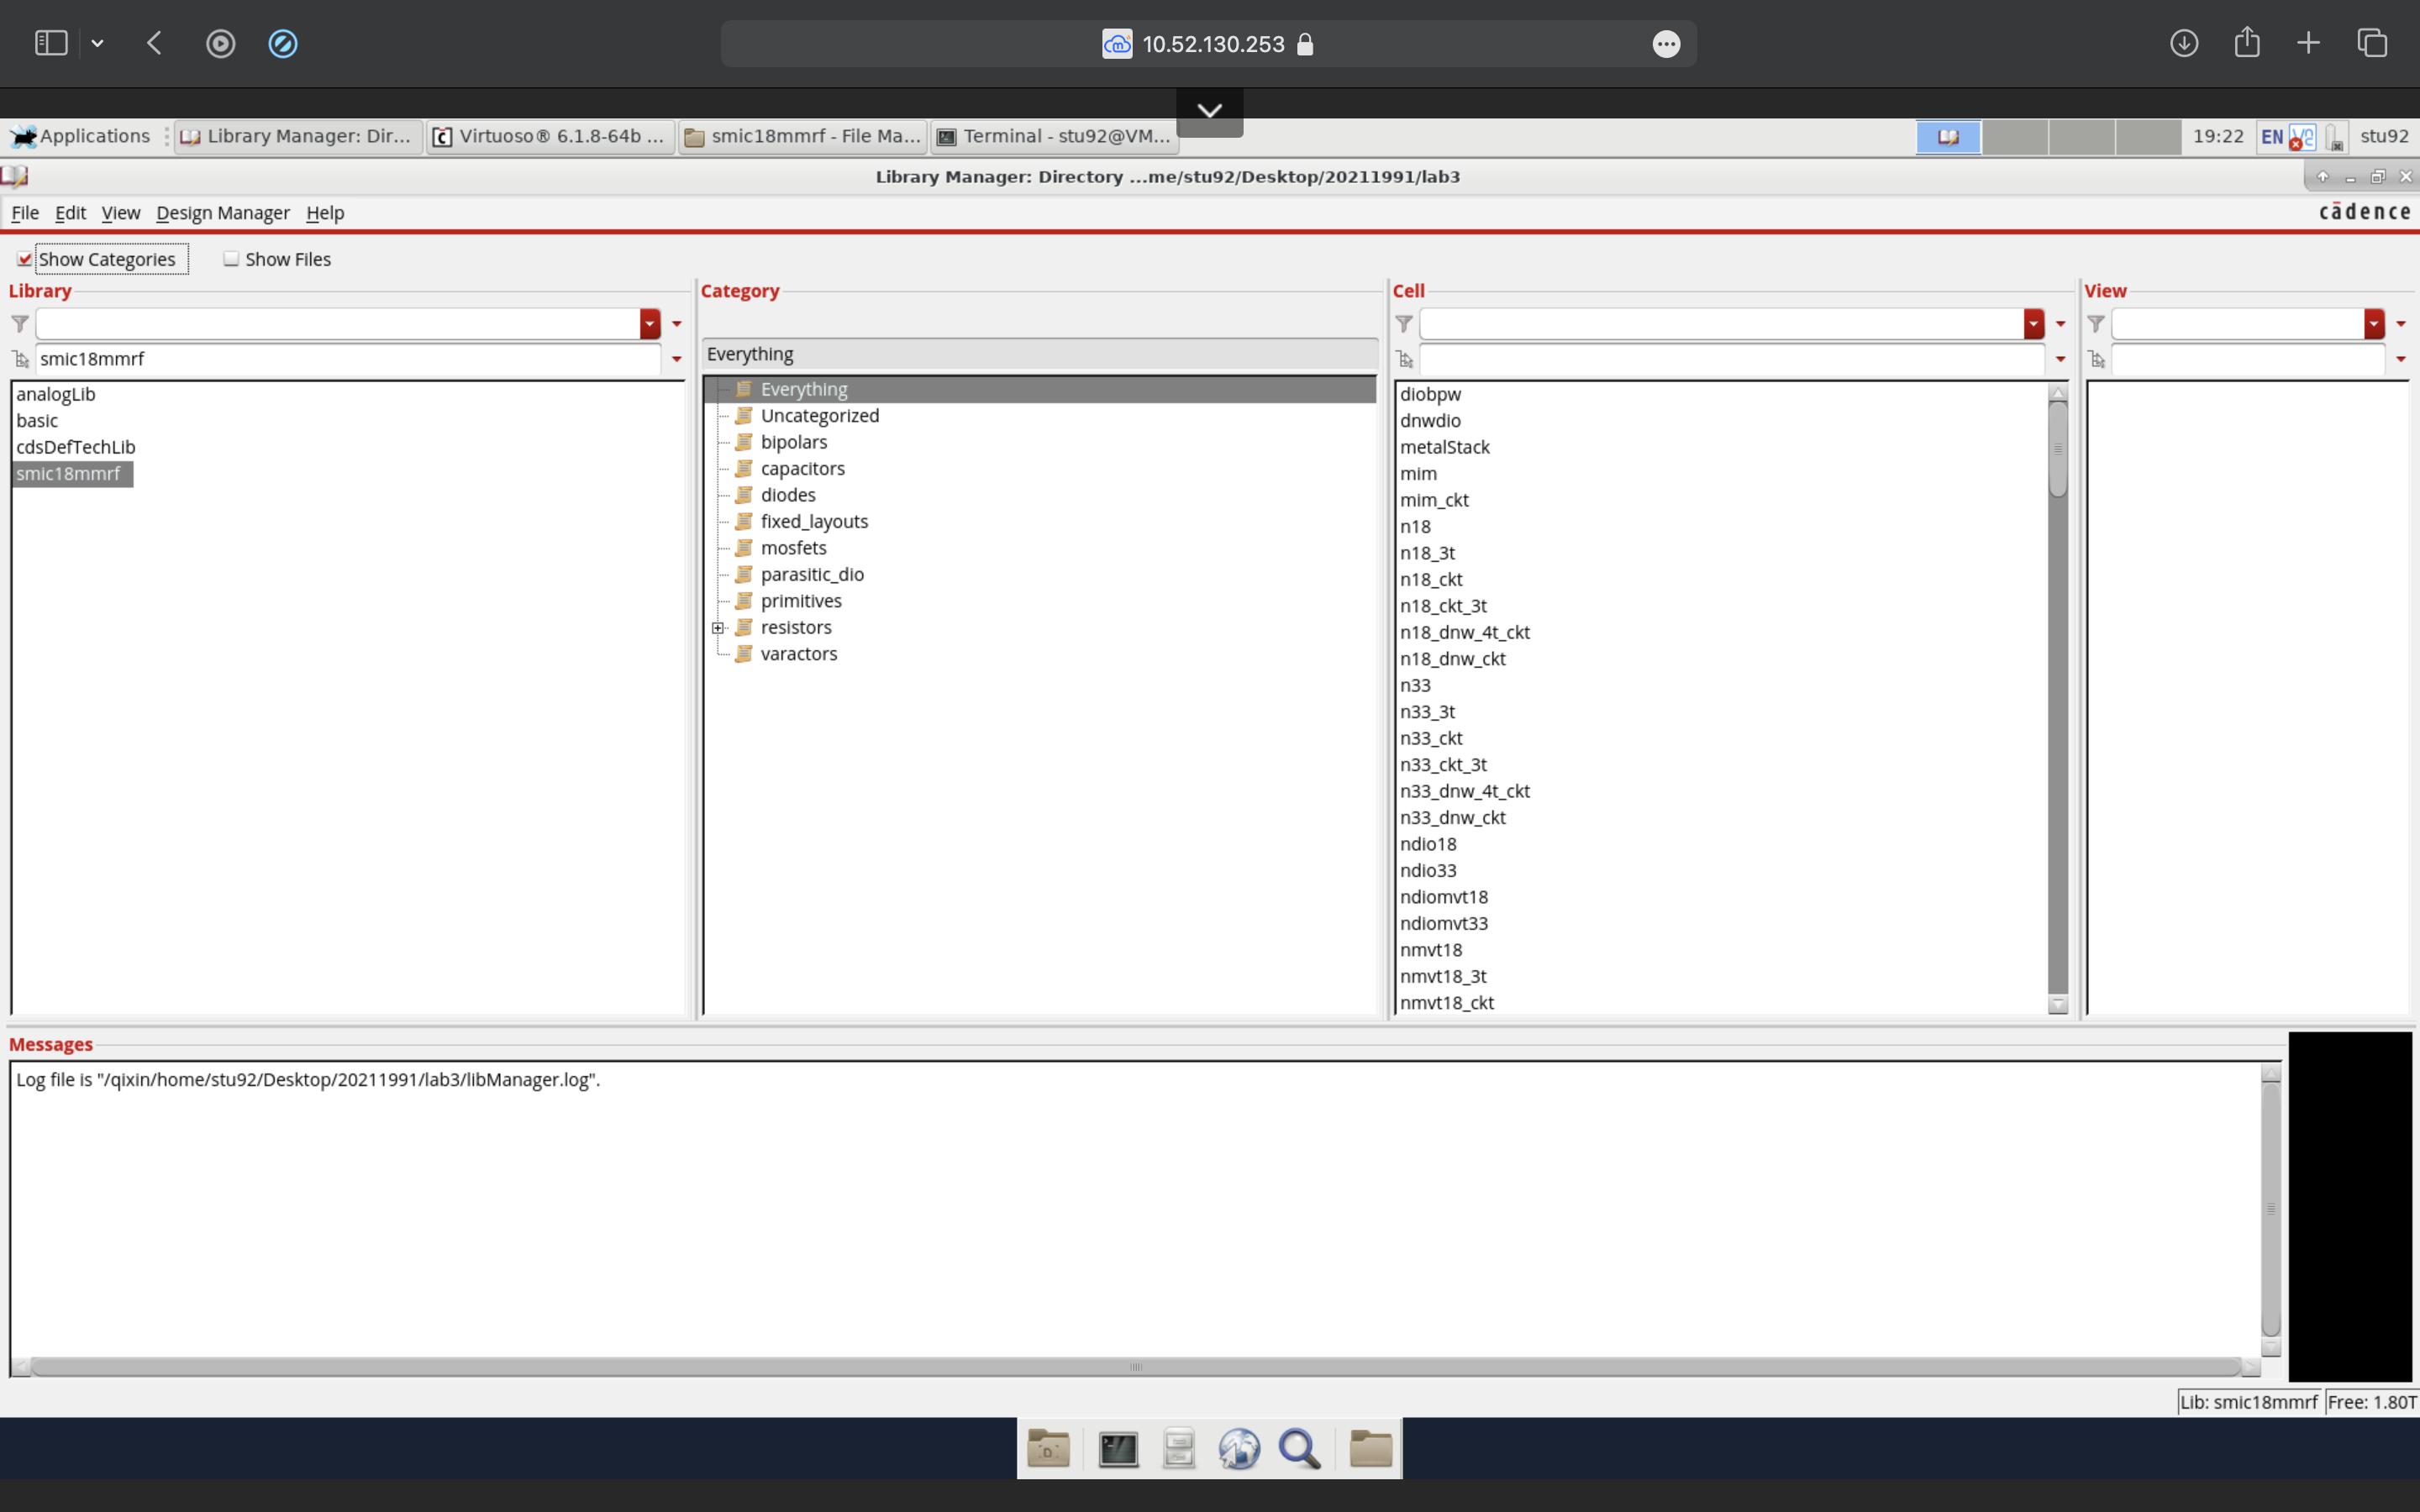
\includegraphics[width=0.9\textwidth]{1-prepare/library-manager.png}
      \caption{library manager}
  \end{minipage}
  \centering\begin{minipage}[t]{0.48\textwidth}
      \centering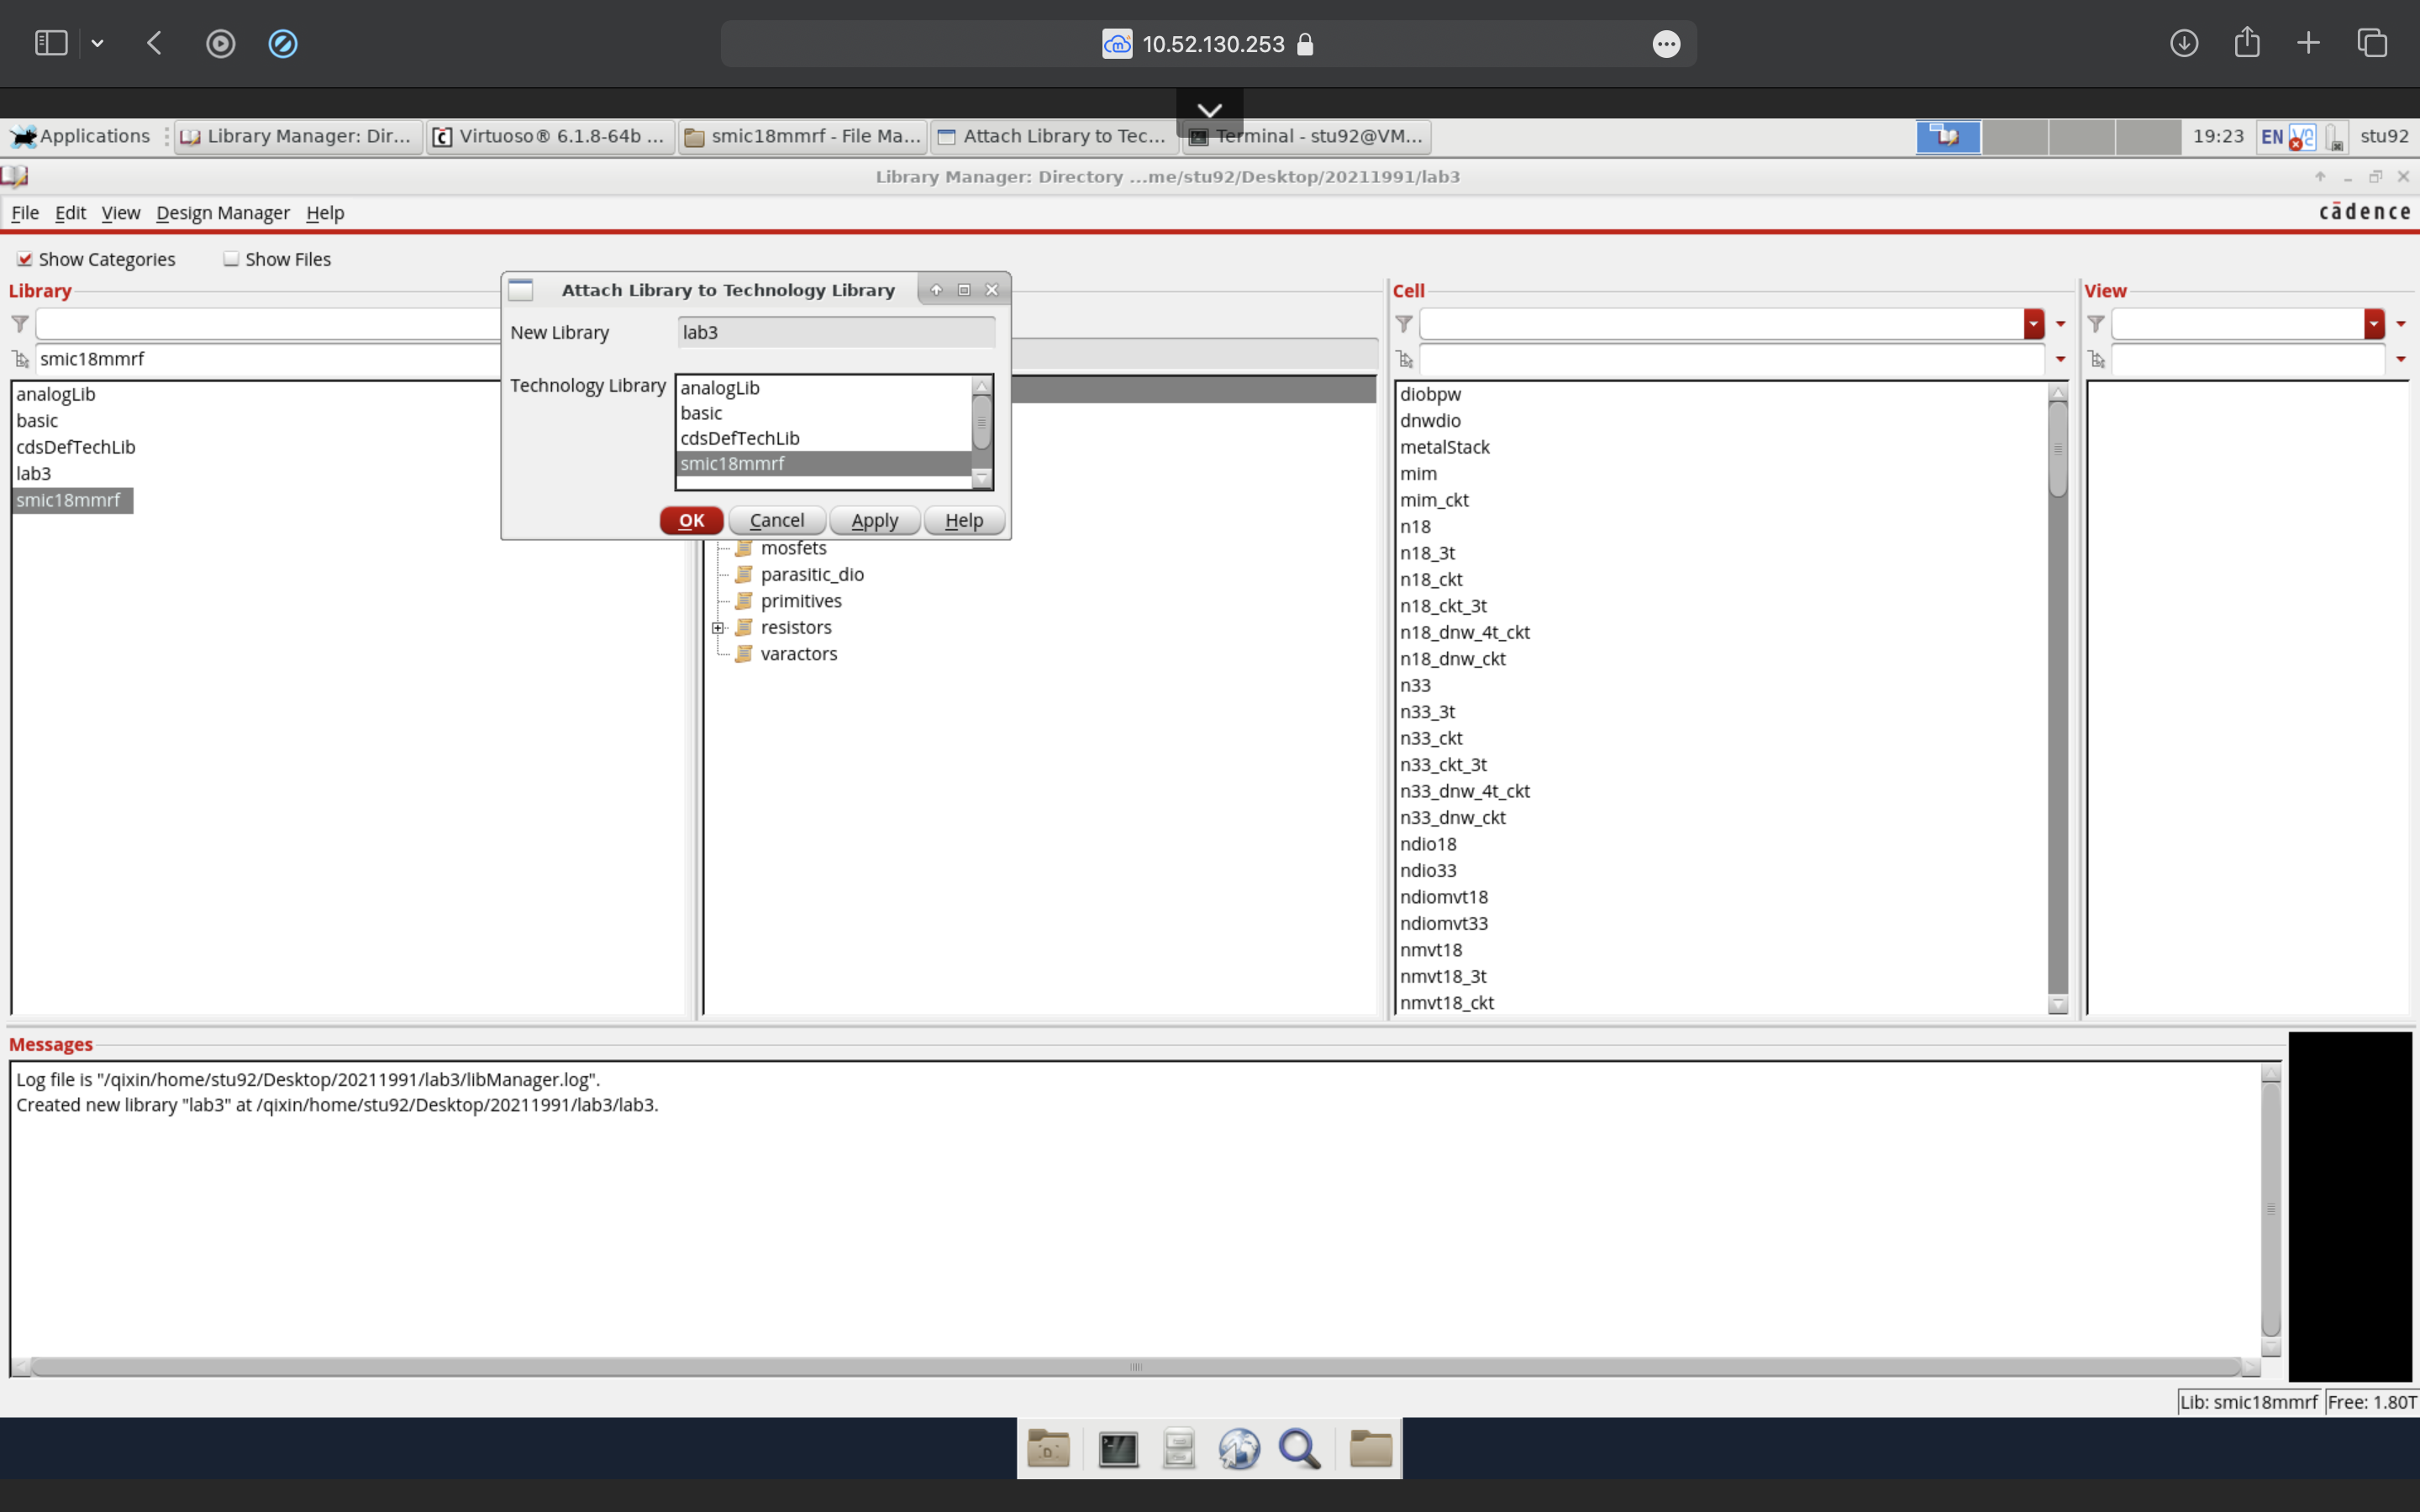
\includegraphics[width=0.9\linewidth]{1-prepare/create-new-library-attach.png}
      \caption{attach technology library}
  \end{minipage}
\end{figure}

\subsubsection{反相器的原理图(schematic)}

设置 n18 和 p18 的参数

\begin{figure}[htbp]
  \centering\begin{minipage}[t]{0.48\textwidth}
      \centering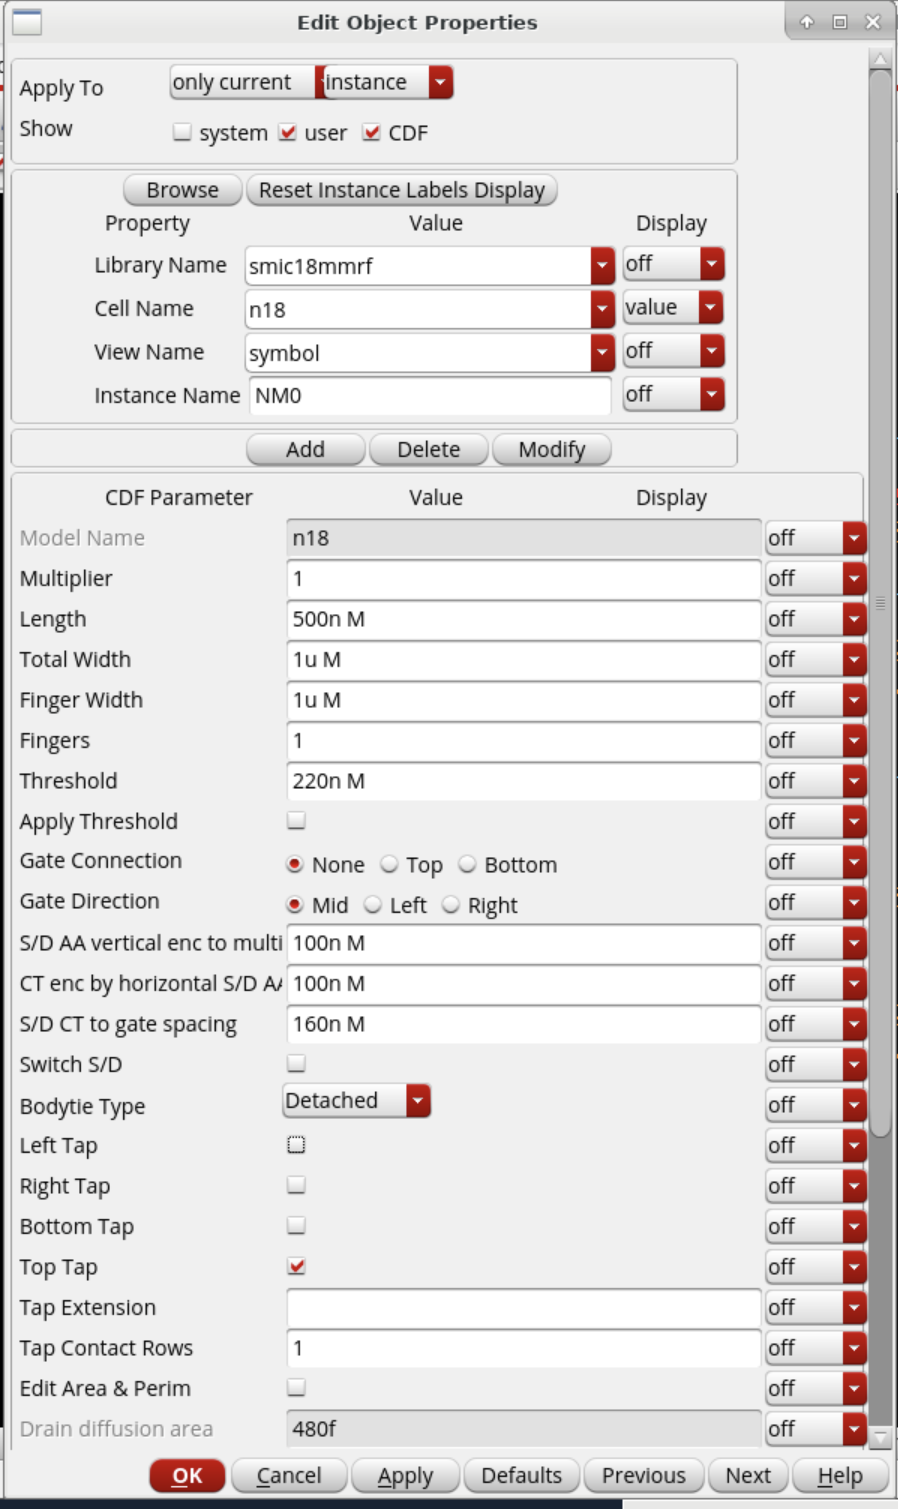
\includegraphics[width=0.9\textwidth]{2-inverter-schematic/para-n18.png}
      \caption{n18}
  \end{minipage}
  \centering\begin{minipage}[t]{0.48\textwidth}
      \centering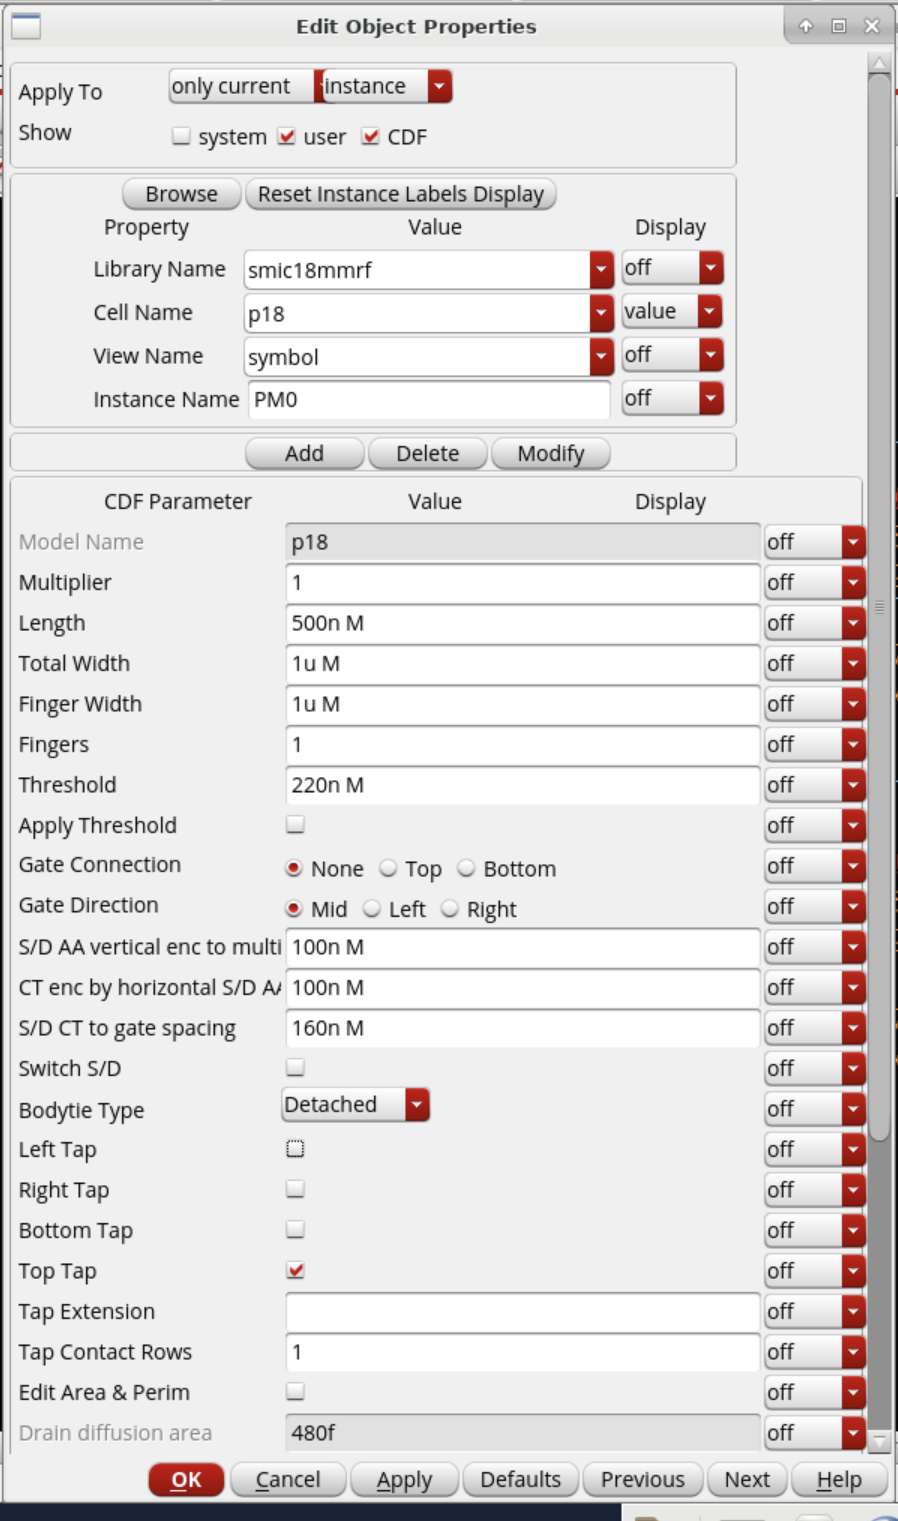
\includegraphics[width=0.9\linewidth]{2-inverter-schematic/para-p18.png}
      \caption{p18}
  \end{minipage}
\end{figure}

下面是最终的反相器原理图

\begin{figure}[H]
  \centering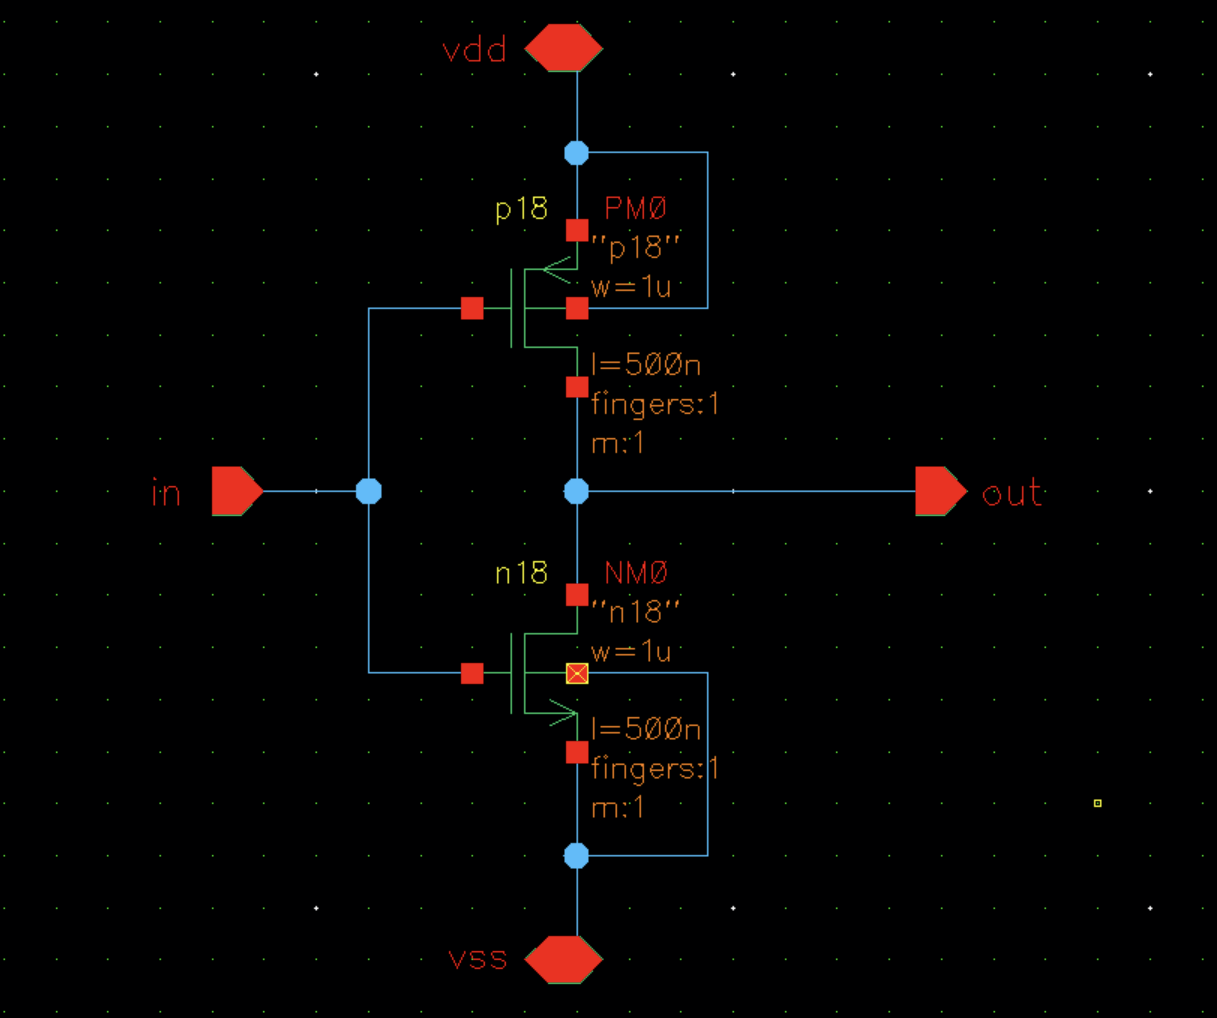
\includegraphics[width=0.6\linewidth]{2-inverter-schematic/inverter-schematic.png}
  \caption{inverter schematic}
\end{figure}

\subsubsection{反相器的版图(layout)}

按照下图进行设置,生成版图

\begin{figure}[H]
  \centering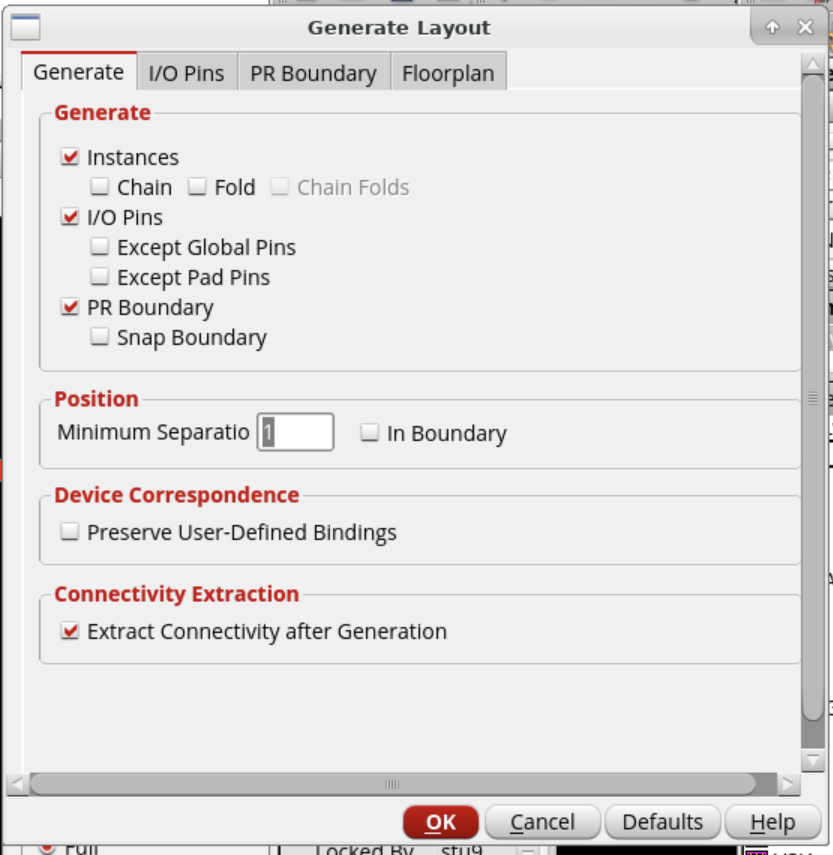
\includegraphics[width=0.6\linewidth]{3-inverter-layout/generate-layout-setting.png}
  \caption{click generate all from source}
\end{figure}

下面是最终的反相器版图

\begin{figure}[H]
  \centering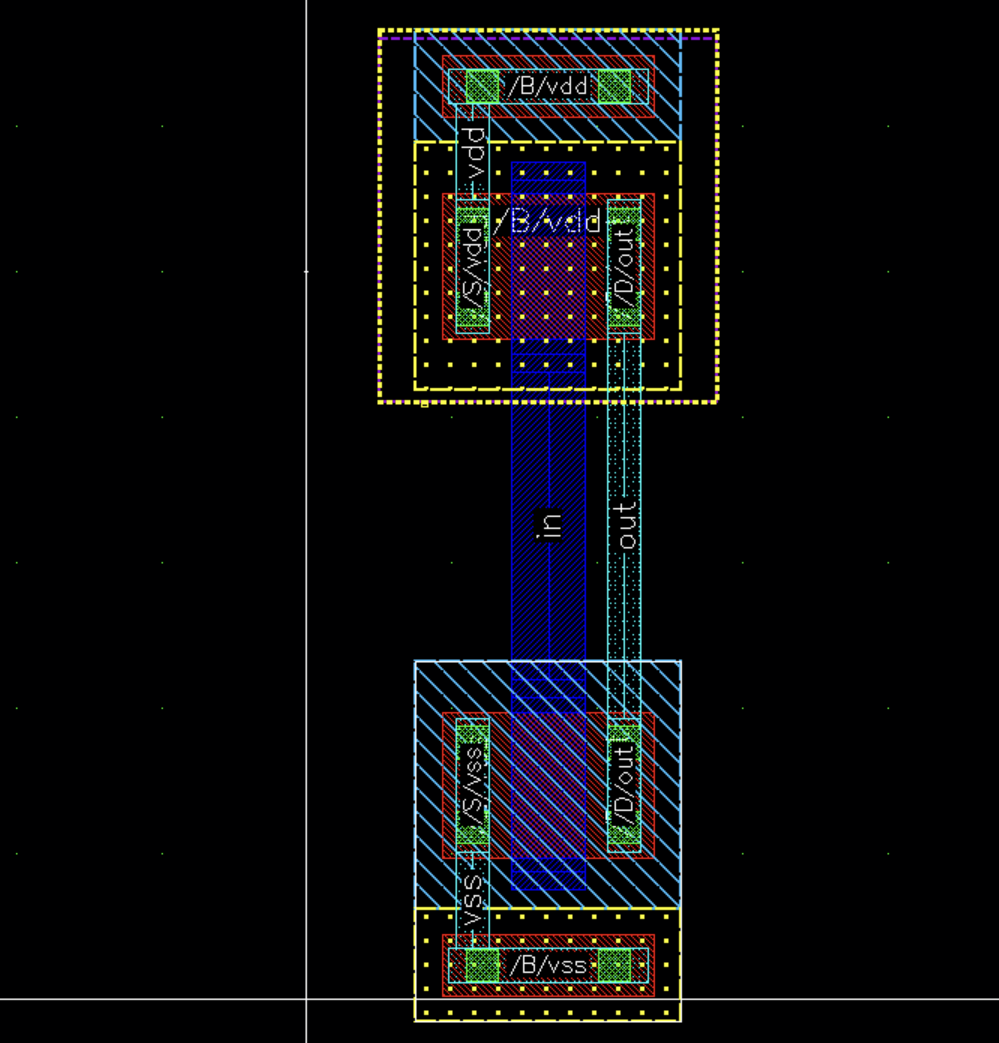
\includegraphics[width=0.6\linewidth]{3-inverter-layout/inverter-layout.png}
  \caption{inverter layout}
\end{figure}

\subsection{反相器的DRC检查}

按照下图进行设置,选择 DRC 检查规则文件

\begin{figure}[H]
  \centering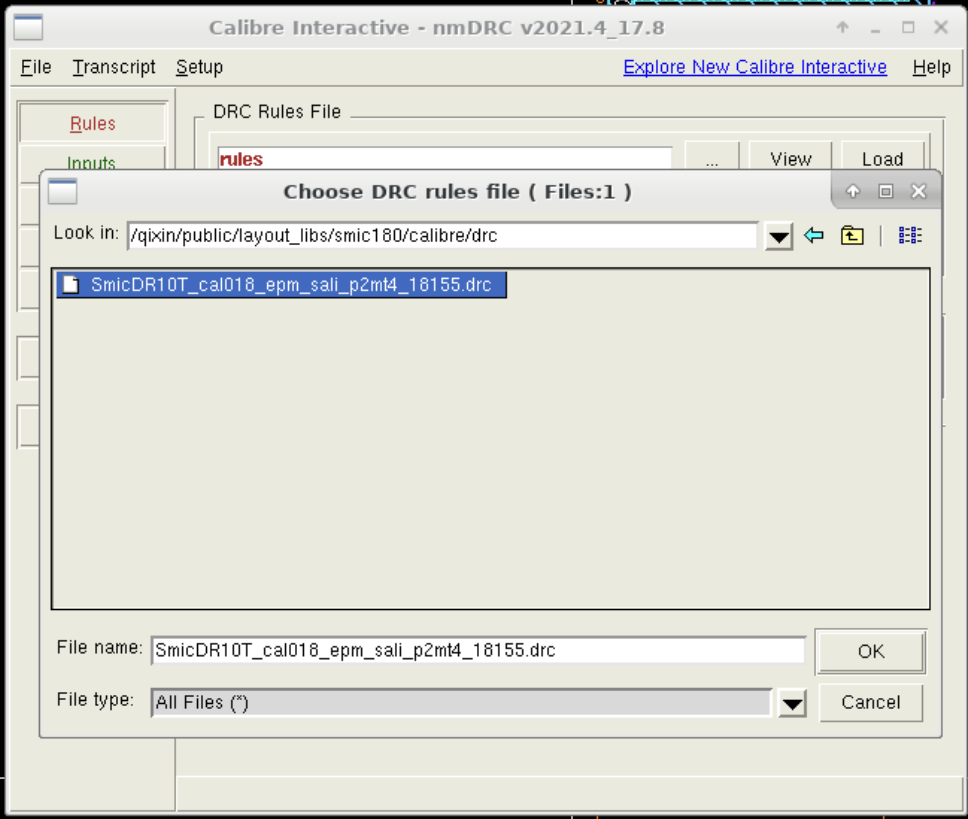
\includegraphics[width=0.6\linewidth]{4-inverter-drc/choose-drc-rules-file.png}
  \caption{choose drc rules file}
\end{figure}

按照下图进行设置,设置 inputs 和 outputs

\begin{figure}[htbp]
  \centering\begin{minipage}[t]{0.48\textwidth}
      \centering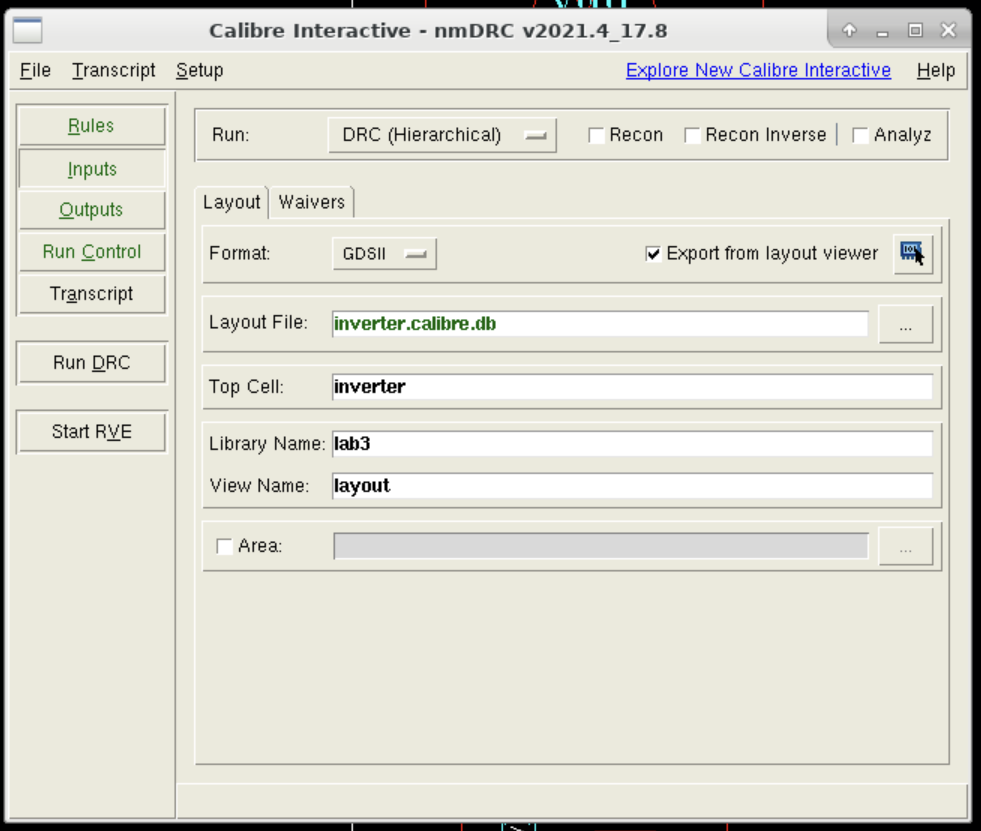
\includegraphics[width=0.9\textwidth]{4-inverter-drc/drc-inputs.png}
      \caption{drc inputs}
  \end{minipage}
  \centering\begin{minipage}[t]{0.48\textwidth}
      \centering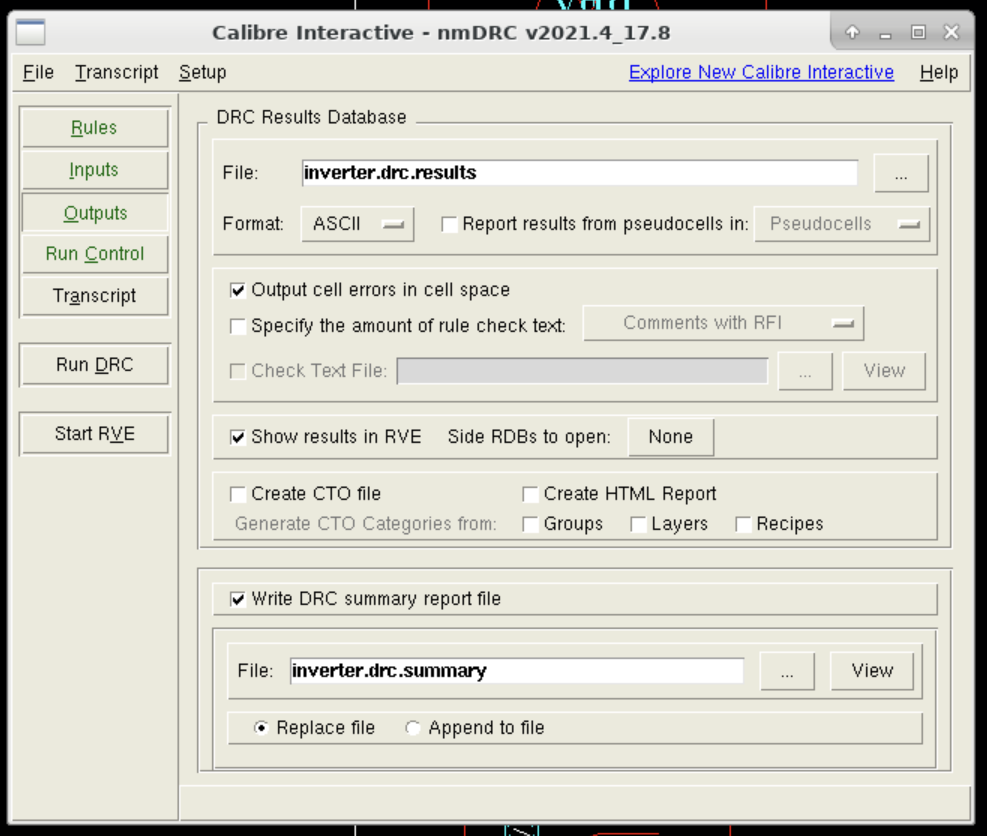
\includegraphics[width=0.9\linewidth]{4-inverter-drc/drc-outputs.png}
      \caption{drc outputs}
  \end{minipage}
\end{figure}

点击 \texttt{Run DRC} 进行 DRC 检查

按照PPT中的提示,对 Layout 进行调整后,最终的 DRC 检查结果如下

\begin{figure}[H]
  \centering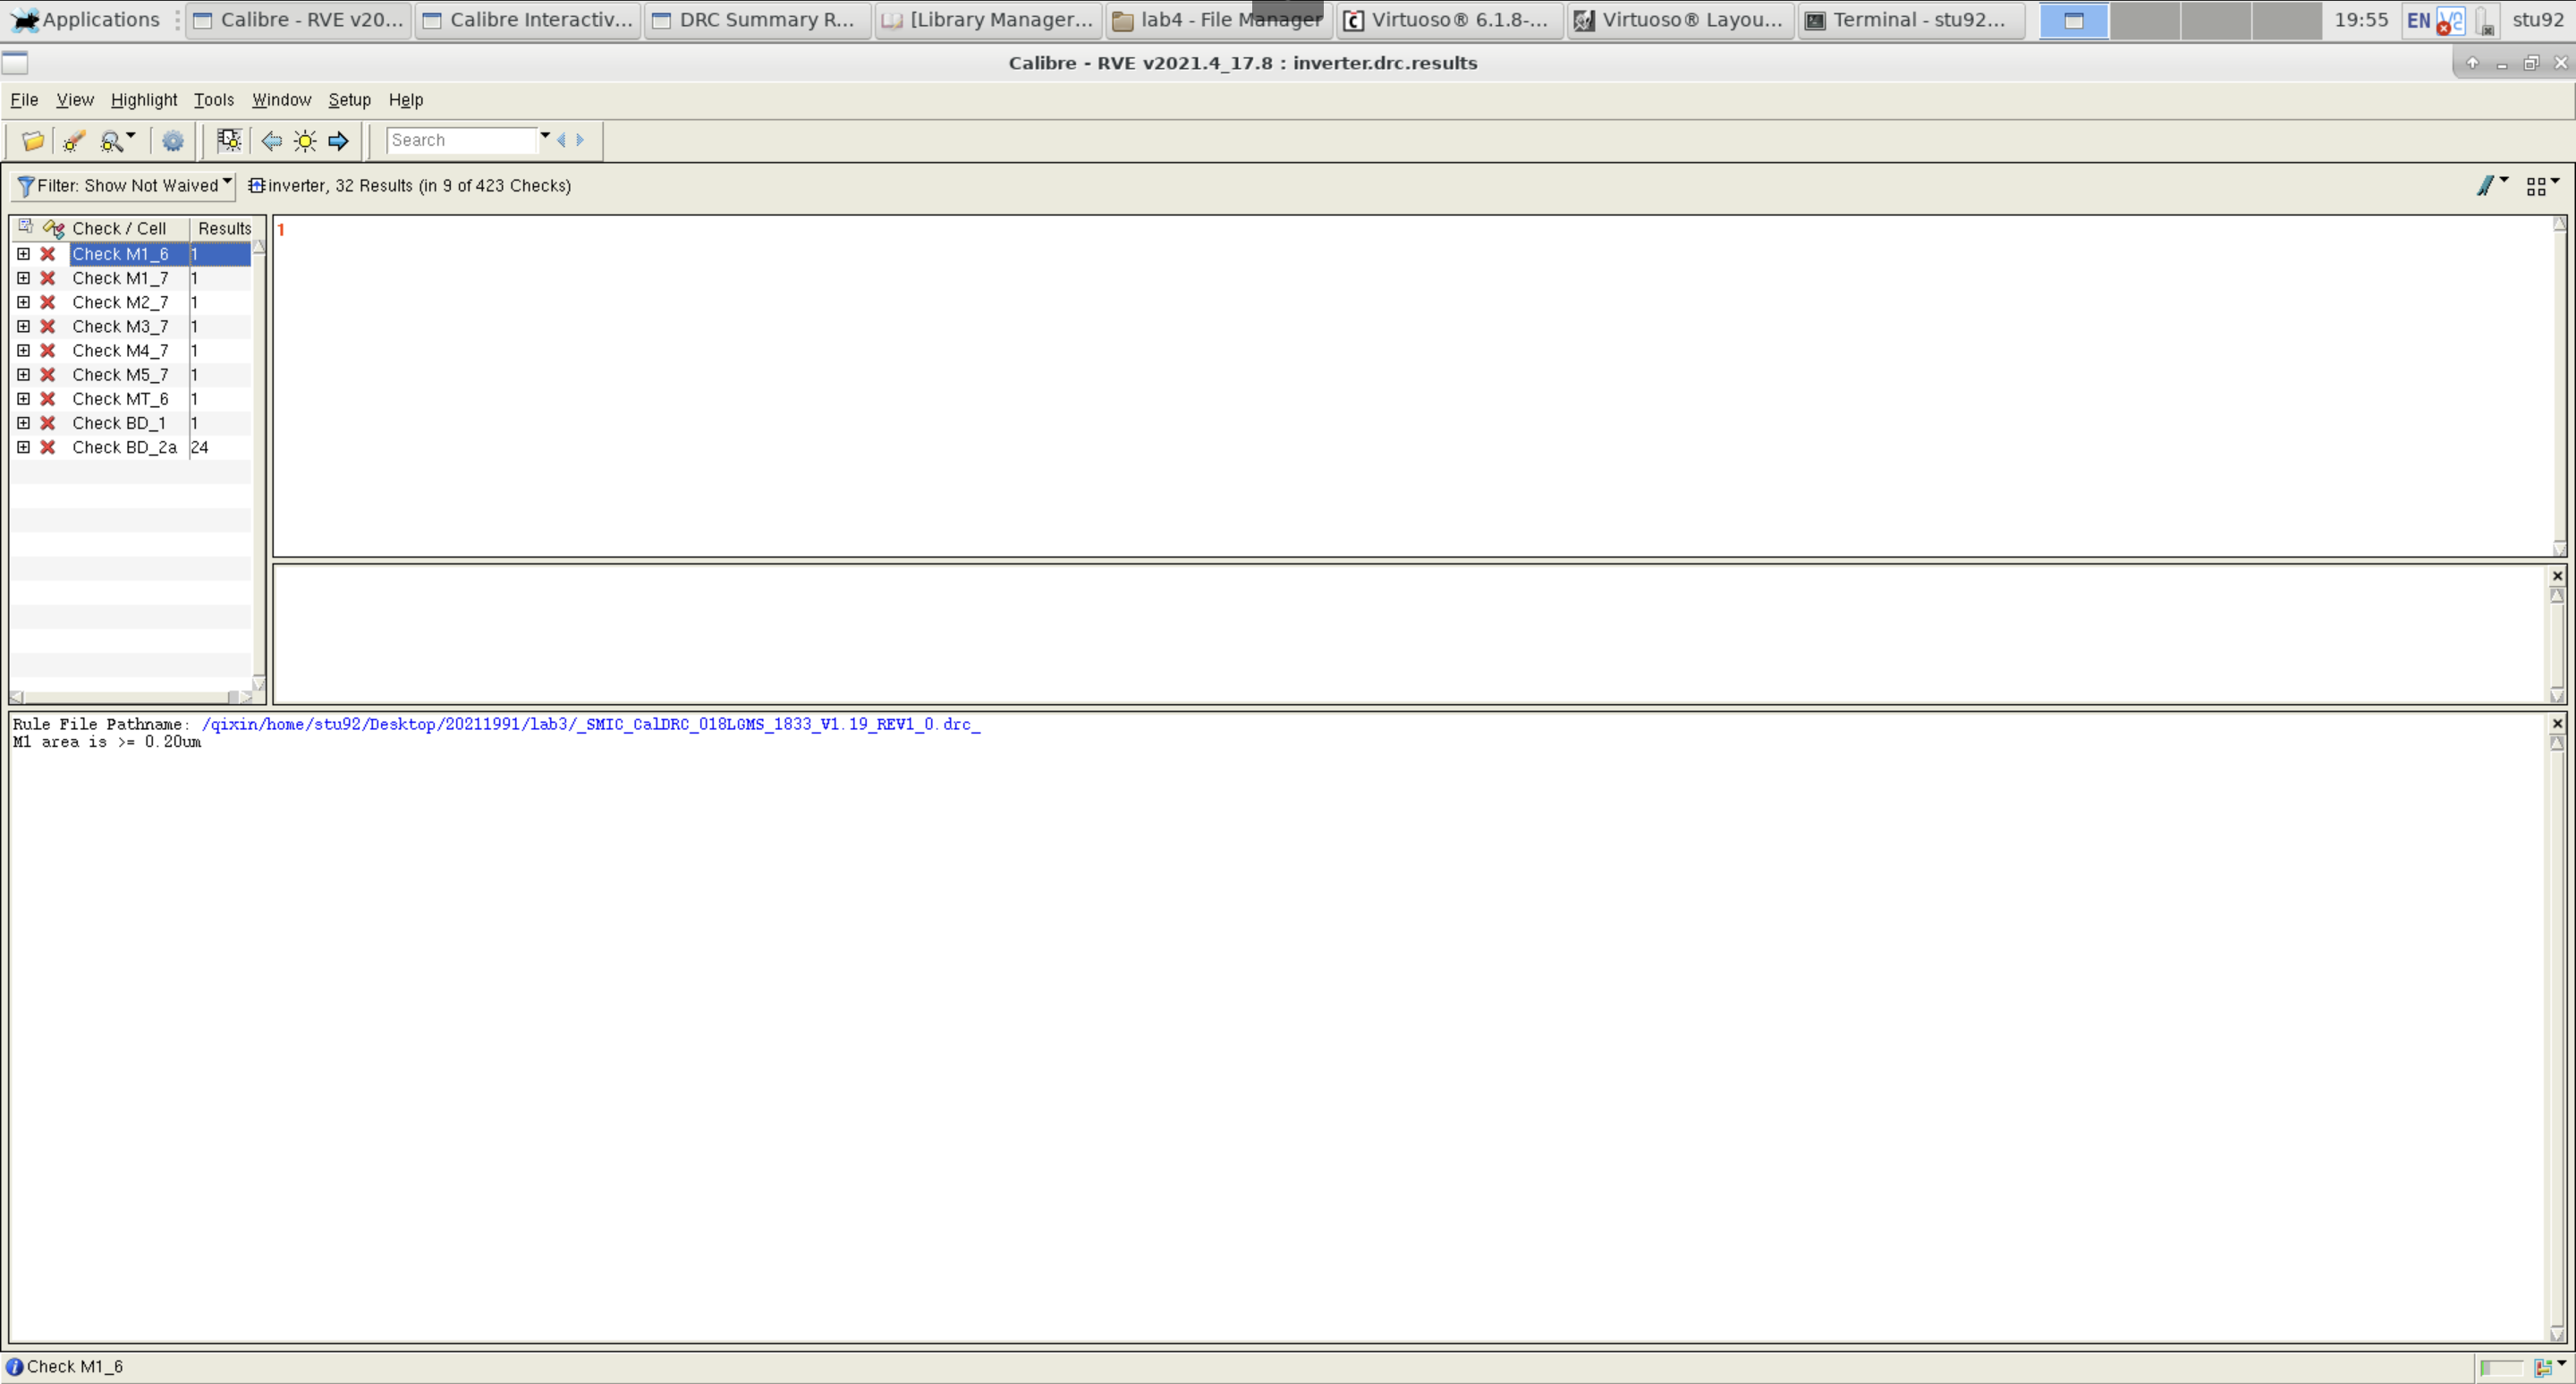
\includegraphics[width=0.6\linewidth]{4-inverter-drc/inverter-drc-2.png}
  \caption{inverter drc}
\end{figure}

\subsection{反相器的LVS检查}

按照下图进行设置,选择 LVS 检查规则文件

\begin{figure}[H]
  \centering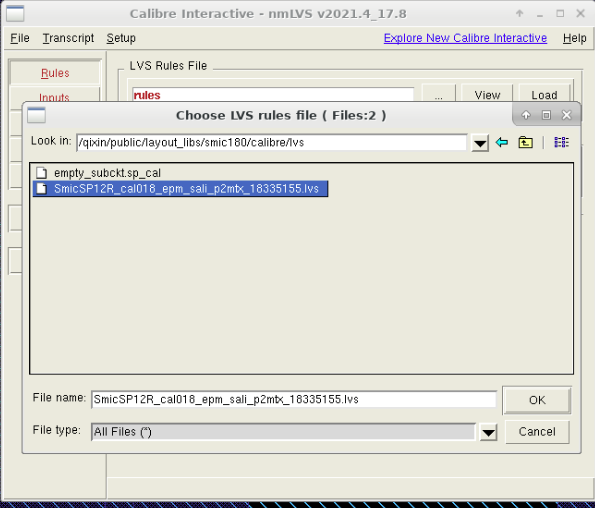
\includegraphics[width=0.6\linewidth]{5-inverter-lvs/choose-lvs-rules-file.png}
  \caption{choose lvs rules file}
\end{figure}

按照下图进行设置,设置 inputs 和 outputs

\begin{figure}[htbp]
  \centering\begin{minipage}[t]{0.48\textwidth}
      \centering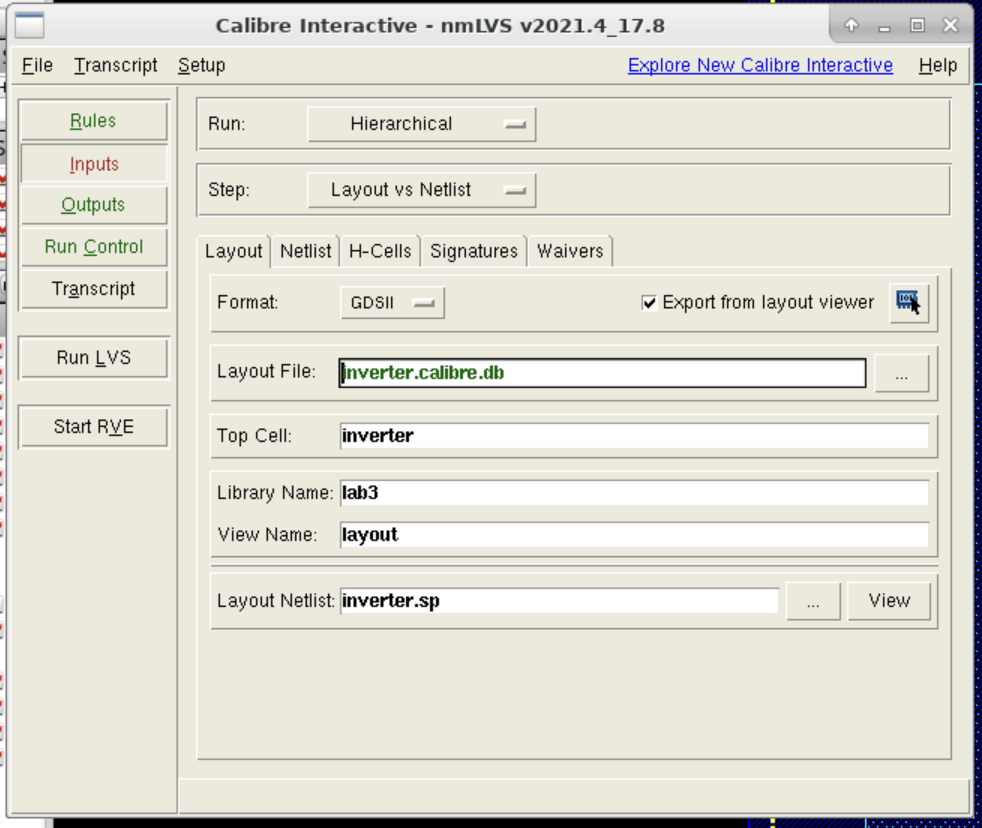
\includegraphics[width=0.9\textwidth]{5-inverter-lvs/lvs-inputs-1.png}
      \caption{lvs inputs}
  \end{minipage}
  \centering\begin{minipage}[t]{0.48\textwidth}
      \centering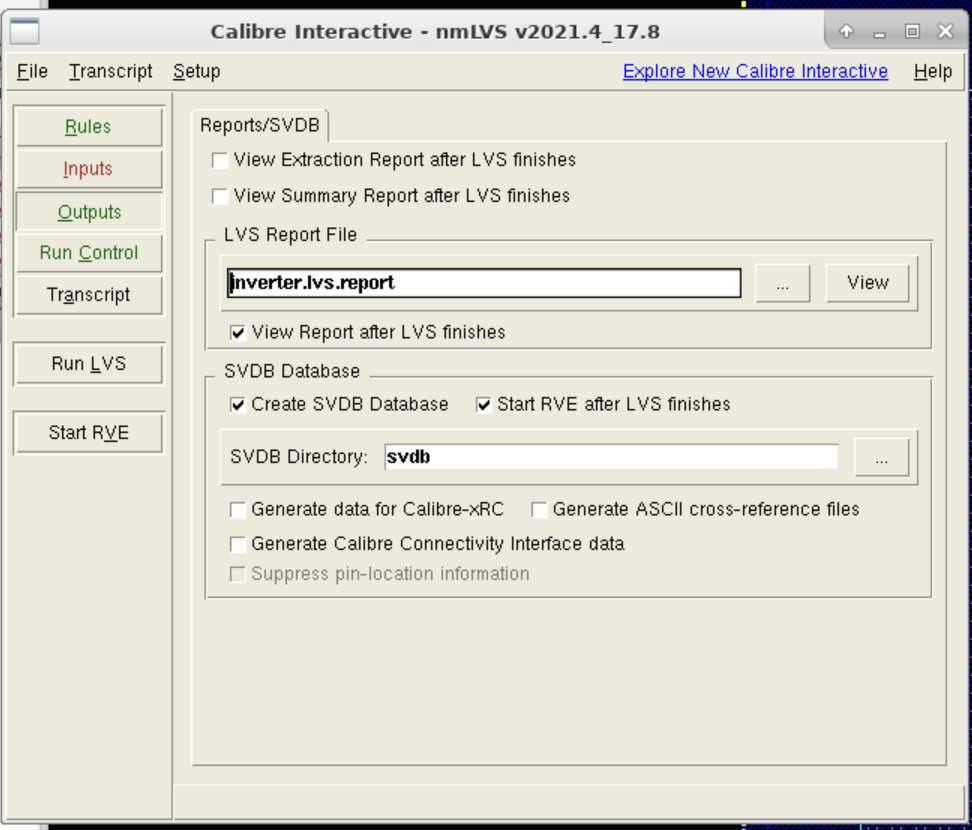
\includegraphics[width=0.9\linewidth]{5-inverter-lvs/lvs-outputs.png}
      \caption{lvs outputs}
  \end{minipage}
\end{figure}

点击 \texttt{Run LVS} 进行 LVS 检查

最终的 LVS 检查结果如下

\begin{figure}[H]
  \centering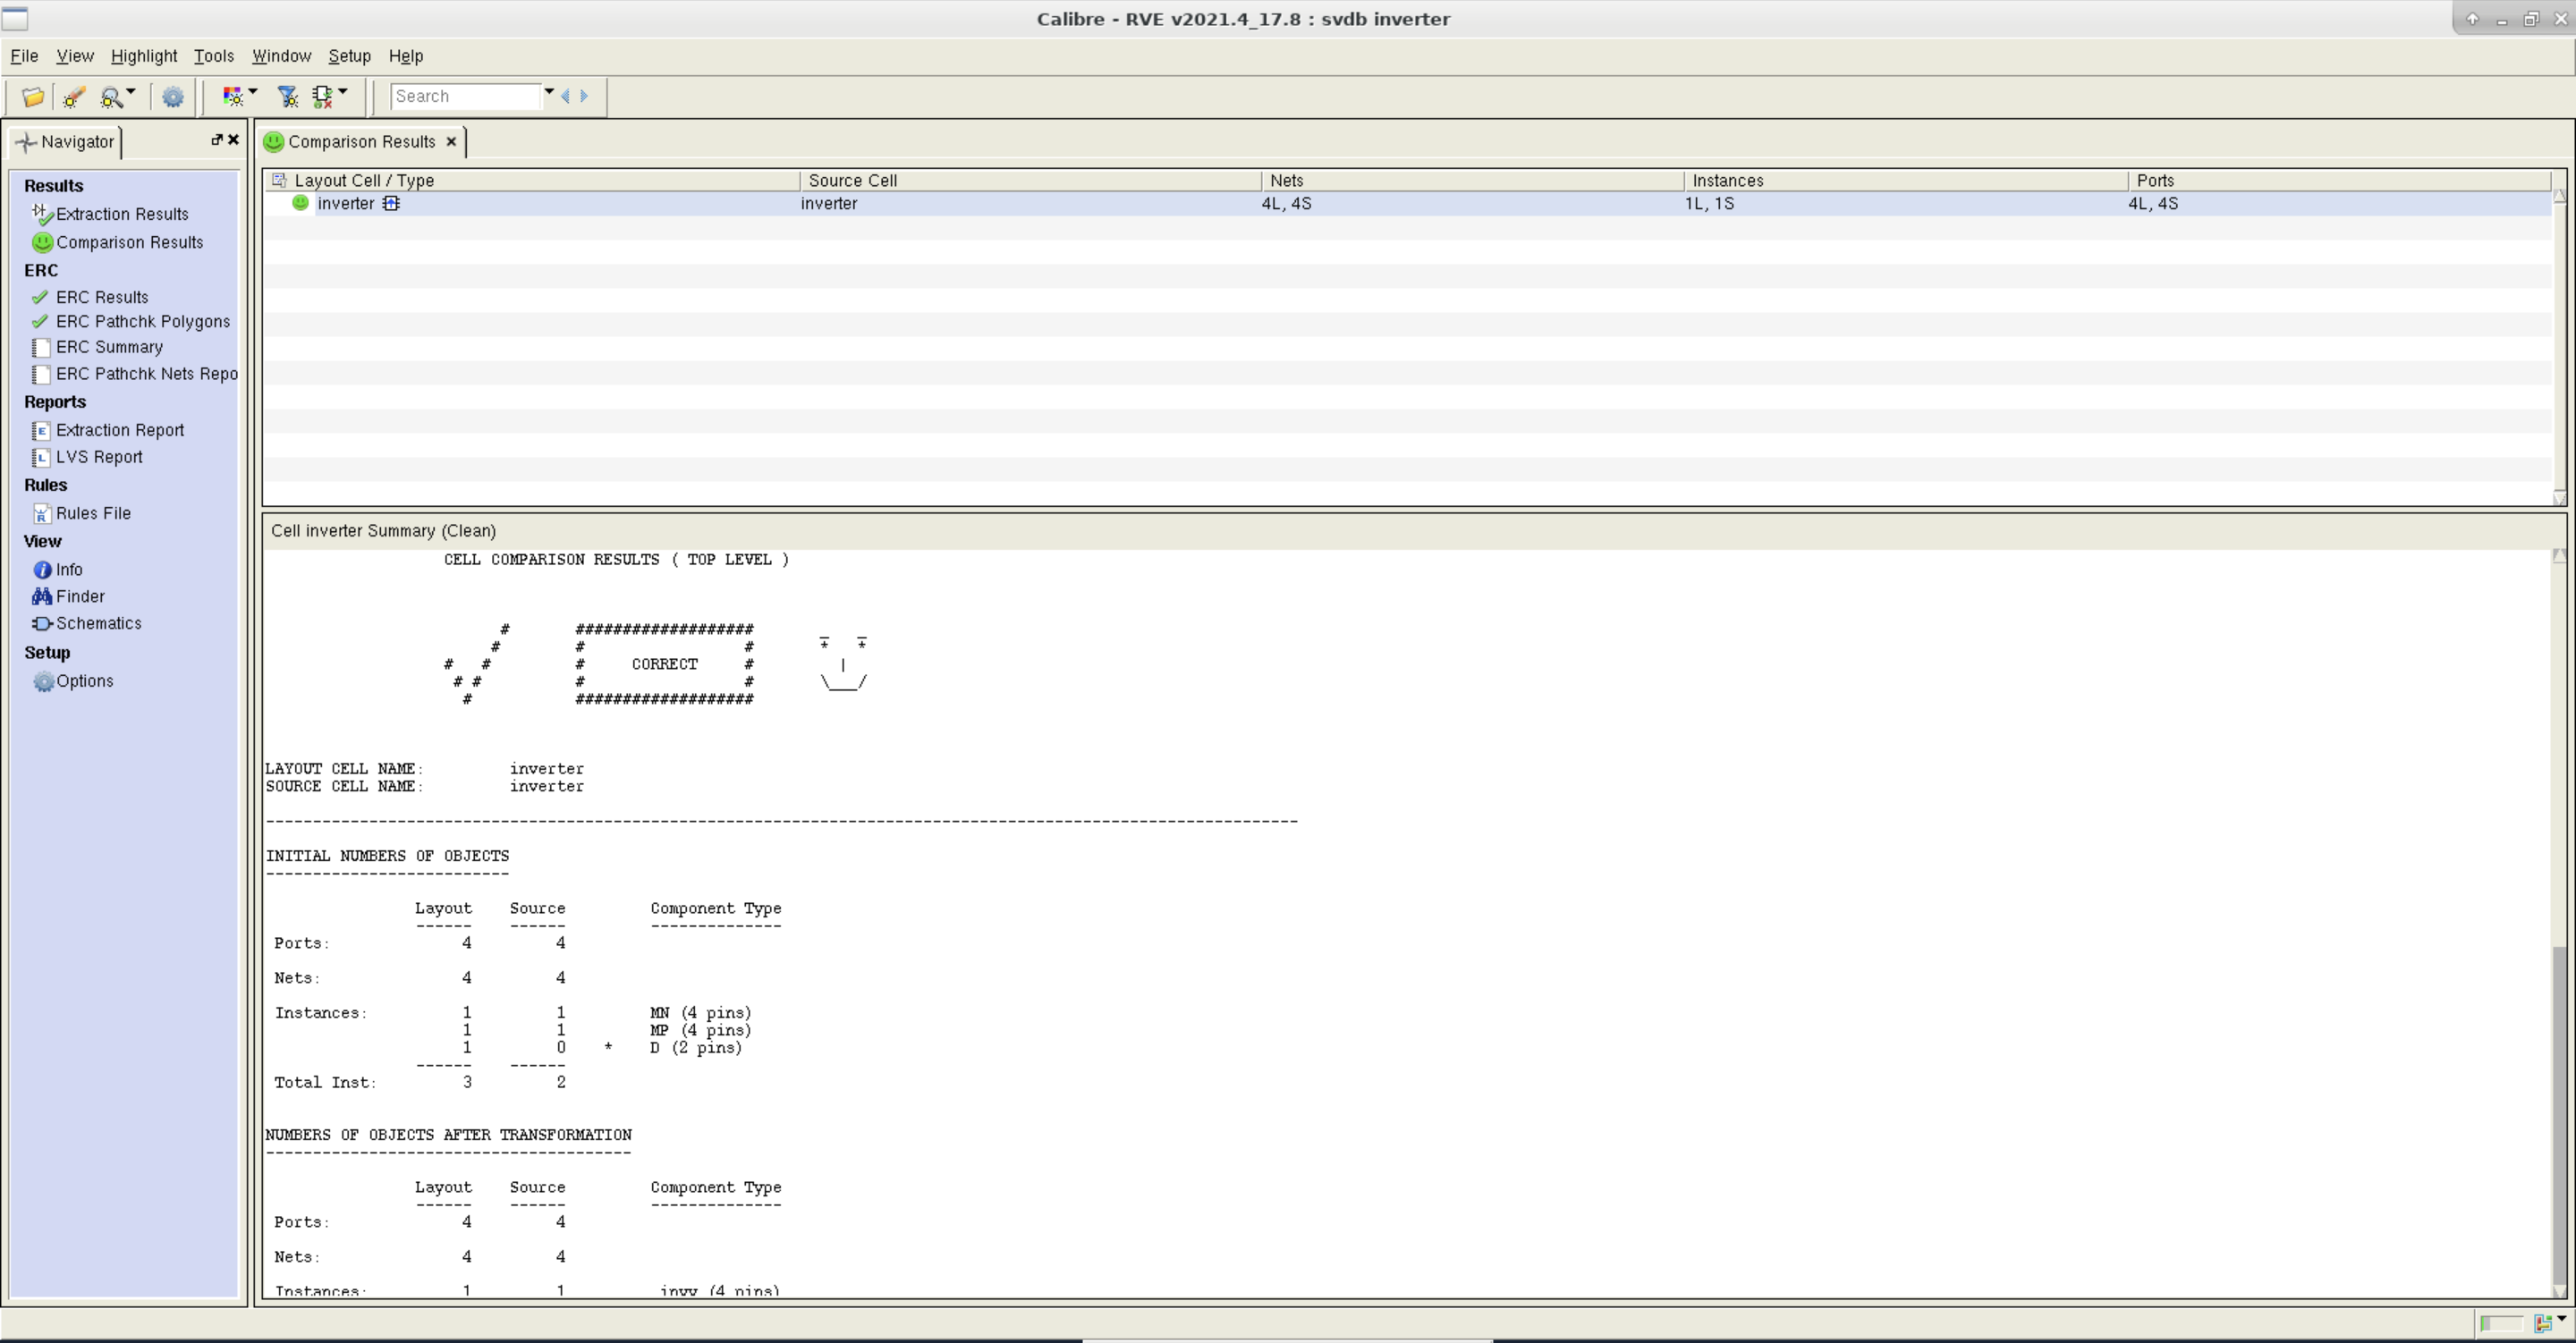
\includegraphics[width=0.6\linewidth]{5-inverter-lvs/inverter-lvs.png}
  \caption{inverter lvs}
\end{figure}

\section{实验总结和感悟}

通过本次实验,我学会了使用 Cadence Virtuoso Editing 进行 CMOS 反相器版图设计,并进行 DRC 和 LVS 检查。在实验中,我遇到了一些问题,比如在进行 DRC 检查时,发现了一些错误,需要对版图进行调整。通过这些问题,我对 CMOS 反相器的设计有了更深入的理解,也对版图设计有了更多的经验。

\end{document}
